\chapter{Related Work and Background}

\section{Related Work}
Researchers are paying increasing attention to methods of scheduling queries optimally on cloud. In this section, we describe the existing literatures relating to our problem of interest.

iCBS \cite{chi2011icbs} offers a generalized profit aware heuristic for ordering queries, but the algorithm considers
assignments to a single VM, and performance goals are limited to
piecewise-linear functions. In \cite{chi2011sla}, they propose a data structure to support profit-oriented workload allocation decisions, including scheduling and provisioning. They consider the problem of mapping each tenant (customer) to a single physical machine to meet performance goals, but ordering and scheduling queries is left to the application.


SmartSLA \cite{xiong2011intelligent} offers a dynamic resource allocation approach for multi-tenant databases. Our model supports a wider range of metrics than the above systems and its decision models offers holistic solutions that indicate the VMs to provision, query assignments, and query execution order. Further the supervised learning model also learns decision models for various SLA types, as opposed to utilizing a hand-written, human-tailored heuristic. This brings an advantage of increased flexibility (changing performance goals without reimplementation) at the cost of some training overhead.

In \cite{tozer2010q,xiong2011activesla}, they propose admission control solutions that reject queries that might cause an SLA violation at runtime, whereas
our system seeks to minimize the cost of scheduling every query
and to inform the user of performance/cost trade-offs. Even if a
query cannot be processed profitably, our model will still attempt
to place it in a cost-minimal way.

Finally\cite{hwang2012minimizing} proposes a system for scheduling Hadoop\cite{maryland1996hadoop} jobs on clouds which takes resource provisioning and deadlines into account. However, it considers only simple per-task deadlines and is not easily generalized beyond Hadoop.
%%%%
\section{Background}
Our system is designed for data management applications deployed on an Infrastructure-as-a-Service (IaaS) cloud. These providers typically offer virtual machines (VMs) of different types for a certain fee per renting period. We assume this deployment is realized by renting VMs with preloaded database engines (e.g., PostgreSQL) and that queries can be executed locally on any of the rented VMs. This property is offered by fully replicated databases.
\subsection{Workload Specification}
Applications begin their interaction with our system by providing a workload specification indicating the query templates  that will compose their workloads. In analytical applications, incoming queries are generally instances of a small number of templates, and queries of the same template have similar performance properties (i.e., latency) because they access and join the same tables. In practice, our approach is agnostic to the tables accessed or joined and cares only about the latency of each template, i.e., queries with identical latency can be treated as instances of the same template. 
\subsection{Performance Goals}
Applications also specify their performance goals for their workloads as functions of query latency. Performance goals can be defined either at the query template level or workload level. Currently, we support the following four types of metrics. (1) Per Query Deadline: users can specify an upper latency bound for each query template (i.e., queries of the same template have the same deadline). (2) Max Latency Deadline: the user expresses an upper bound on the worst query response time in a query workload. (3) Average Deadline: sets an upper limit on the average query latency of a workload. (4) Percentile Deadline: specifies that at least x\% of the workload’s queries must be completed within t seconds. These metrics cover a range of performance goals typically used for database applications. Performance goals are expressed as part of a Service-Level-Agreement (SLA) between the IaaS provider and the application that states (a) the workload specification, (b) the performance goal,and (c) a penalty function that defines the penalty to be paid to the application if that goal is not met. Our system is agnostic to the details of the penalty function, incorporating it into its cost-model as a “black box” function that maps performance to a penalty amount. 
\begin{figure}
\centering
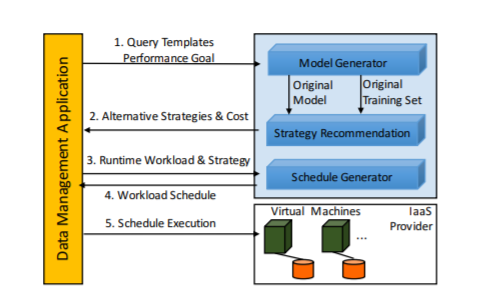
\includegraphics[width=0.9\textwidth]{architecture.PNG}
\caption{\label{fig:Archi}Architecture of the model}
\end{figure}
The architecture of the system is shown in Figure ~\ref{fig:Archi}. Workload and performance specifications are submitted to the system, which trains a model. The training set for this model is also leveraged to generate alternative decision models (strategies) for stricter and more relaxed performance goals (Strategy Recommendation). These strategies are presented to the user along with a cost function that estimates the monetary cost of each strategy based on the frequency of each query template in a given workload.

Given an incoming workload at runtime, the application estimates the expected cost and performance of executing these workloads using our proposed strategies and chooses the one that better balances performance needs and budget constraints (Execution Strategy). Our system identifies (a) the type/number of VMs to be provisioned, (b) the assignment of queries to these VMs and (c) the execution order of the queries within each VM, in order to to execute the incoming workload based on the chosen strategy. This step is executed by the Schedule Generator which can generate these workload schedules. Applications execute their workloads according to the system’s recommendations. They rent VMs as needed and add queries to the processing queue of VMs according to the proposed schedule. 
